\documentclass{article}
\usepackage[utf8]{inputenc}
\usepackage{graphics}
\usepackage{graphicx}
\usepackage{float}
\usepackage[italian]{babel}
\usepackage{hyperref}
\usepackage[section]{placeins}
\title{Homework ISBI}
\author{Giuliano Di Giuseppe matr. M63001322
    \and Raffaele Russo matr. M63001325 
    \and Alessandro Vanacore matr. M63001359}

\date{}

\begin{document}
\maketitle
\tableofcontents
\newpage

\section{Homework 1- Modellazione funzionale}
\subsection{Traccia}
\textit{
Modellare attraverso opportuni diagrammi UML un ente che deve creare un processo di dematerializzazione.}
\subsection{Introduzione}
Si assume che l'organizzazione considerata è costituita da:
\begin{itemize}
    \item Amministrazione generale: identifica i documenti da dematerializzare e li richiede al relativo magazzino locale. Una volta ricevuti, procede con l'archiviazione di quest'ultimi nel database aziendale dopo averli opportunamente formattati e firmati digitalmente.
     \item Magazzini locali: si occupano di ricercare i documenti richiesti e consegnarli alle relative amministrazioni locali.
    \item Amministrazioni locali: si occupano di scannerizzare e inoltrare all'amministrazione generale i documenti conformi.
   
    
\end{itemize}
\subsubsection{Descrizione delle attività}
\begin{itemize}
    \item ACQUISIZIONE INFORMAZIONI DOCUMENTI: l'amministrazione generale richiede informazioni inerenti alla locazione e all'ID dei documenti da comunicare al magazzino.
    \item RICHIESTA DOCUMENTI: il sistema inoltra al relativo magazzino locale una richiesta, contenente tutte le informazioni riguardanti i documenti da scannerizzare.
    \item RICERCA FASCICOLI: l'impiegato cerca i fascicoli richiesti nel magazzino.
    \item CONSEGNA FASCICOLI: si effettua la consegna dei fascicoli all'amministrazione locale.
    \item SCANNERIZZAZIONE FASCICOLI: l'impiegato si occupa di scannerizzare correttamente tutti i fascicoli ricevuti.
    \item CONTROLLO SCANNERIZZAZIONE: l'impiegato controlla la leggibilità del fascicolo scannerizzato. Se la scannerizzazione non è avvenuta correttamente bisogna ripeterla.
    \item INVIO FASCICOLI: si effettua l'invio all'amministrazione generale di tutti i fascicoli scannerizzati.
    \item FORMATTAZIONE DOCUMENTI: i documenti vengono formattati correttamente dall'amministrazione generale.
    \item FIRMA DIGITALE: il documento viene firmato digitalmente.
    \item ARCHIVIAZIONE DATABASE: i dati vengono archiviati in un opportuno database.
\end{itemize}

\subsection{Diagrammi}
\subsubsection{Diagramma dei casi d'uso}
In figura \ref{fig:1} è mostrato il diagramma dei casi d'uso relativo al processo di dematerializzazione dei documenti.

\begin{figure}[H]
    \centering
    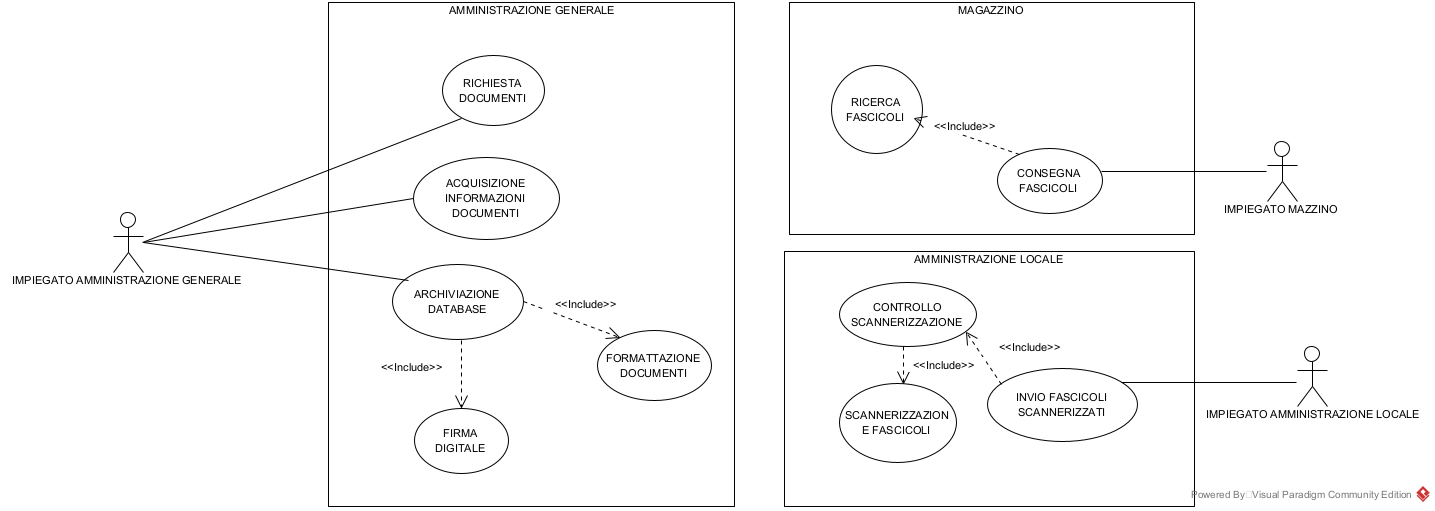
\includegraphics[scale=0.3]{Homework1 - Diagramma dei casi d'uso.png}
    \caption{Diagrama dei casi d'uso}
    \label{fig:1}
\end{figure}

\subsubsection{Diagramma di attività}
In figura \ref{fig:2} è mostrato il diagramma di attività relativo al processo di dematerializzazione dei documenti.
\begin{figure}[H]
    \centering
    \includegraphics[scale=0.3]{Homework1 - Diagramma di attività.png}
    \caption{Diagramma di attività}
    \label{fig:2}
\end{figure}

\subsection{Approfondimento sicurezza}
Possiamo rendere il processo di dematerializzazione robusto a eventuali attacchi informatici del tipo man in the middle e preservare l'integrità e la riservatezza delle informazioni trasmesse. A tal proposito si può pensare che ogni magazzino locale abbia una propria funzione di hash con cui generare un digest da concatenare al documento scannerizzato. Si procede poi a crittografare l'intero messaggio secondo uno schema con chiave simmetrica, propria di quel magazzino. Il messaggio ricevuto viene decifrato dall'amministrazione generale, che ne verifica l'integrità, effettuando un controllo del digest. Succesivamente si utilizzerà un sistema di cifratura del tipo AES-256 prima di archiviare le informazioni nel database. 


\end{document}
